
\documentclass[aoas,preprint]{imsart}

\usepackage[english]{babel}
\usepackage[T1]{fontenc}
\usepackage{amsbsy,alltt,amsmath,times, amsthm, amssymb, latexsym}
\usepackage{color, graphicx, rotate, colordvi, comment, url}
\usepackage{amsbsy}
\usepackage{amsmath}
\usepackage{amssymb}
\usepackage{latexsym}
\usepackage{graphicx}
\usepackage{comment}
\usepackage{rotating}
\usepackage{epsfig, color, graphicx, rotate, colordvi}
\usepackage{url}
\usepackage{hyperref}
\usepackage{amsfonts}
\usepackage{subfigure}
\usepackage{bm}
\usepackage{multirow}

\startlocaldefs
\endlocaldefs

\begin{document}

\begin{frontmatter}


\title{Does considerable loss in income late in life cause
an increase in all-cause mortality?
}
\runtitle{Negative Wealth Shock and All-Cause Mortality}

\author{\fnms{Hanying} \snm{Jiang}\ead[label=e1]{hjiang252@wisc.edu}},
\author{\fnms{Peng} \snm{Yu}\ead[label=e2]{pyu58@stat.wisc.edu}}
\and
\author{\fnms{Taiyu} \snm{Ye}
\ead[label=e3]{tye33@stat.wisc.edu}}

\affiliation{Department of Statistics, Universith of Wisconsin-Madison}

\runauthor{H. Jiang et al.}

\begin{abstract}
A negative wealth shock may cause emotional fragility and poor health. The attendant financial problem leads to low quality of life and expenses of health care. Elderly people will be exposed to more risk, become more vulnerable after a large sudden wealth loss and have less probability to return a previous stage. So a negative wealth shock results in potentially long-term, and even permanent, changes in a variety of physiological and psychological factors, and is even associated with mortality. To figure out the effect of considerable loss in income late in life on all-cause mortality rate, we analyze the data from the Health and Retirement Study, a longitudinal panel study that surveys a representative sample of approximately 20,000 people in America. Removing the samples out of our study duration or with too much missing data, we finally used a data set with 10007 samples. After adopting a time-varying balanced risk set matching procedure, the average treatment effect is calculated. We concluded that a negative wealth shock will increase all-cause mortality rate among old people. And this conclusion is robust to unobserved confounders.
\end{abstract}

\begin{keyword}
\kwd{wealth shock}
\kwd{all-cause mortality}
\kwd{time-varying balanced risk set matching}
\end{keyword}

\end{frontmatter}

\section{Introduction}
Money gives access to advanced educational resources, quality life, healthy nutrition and high-level entertainment. The fact that economic resources can influence almost everything is not only believed by most people, but also has been demonstrated by studies. It has been revealed that wealth plays an important role in first marriage entry, people may delay marriage or even be deterred from marrying because of the lack of money\cite{r8,r5}. Poverty causes stress and negative affective states which in turn may lead to short-sighted and risk-averse decision-making, possibly by limiting attention and favoring habitual behaviors at the expense of goal-directed ones\cite{r6}. We can even directly conclude that raising income can increase average long-term happiness\cite{r7}. So it has been a general consensus that richer people tend to be healthier. Although the literature on the relationship between economic resources and health has become substantial, most of them focus on the association between and few researchers consider this problem from the perspective of Cause-effect relationships.

A negative wealth shock, defined as a loss of 75\% or more of total net worth over a 2-year period. We are interested in the effect of negative wealth shock in mortality among old people. However, the positive correlation between negative wealth shock and mortality among old people can be interpreted in several alternative ways. High mortality rate and large sudden losses of net worth could be both caused by diseases. Many people in poor health condition are struggling to pay their medical bills and have accumulated medical debt over time. Their career choices are also limited by the damaged labour power. So diseases could lead to not only higher death rate, but also personal financial crisis. Alternatively, rising mortality risk can be the effect of negative wealth shock. A sudden loss of money is a heavy strike and brings high pressure. The direct consequence is low economic standing and it means no access to better treatment, targeted therapy and expensive medications. Specifically, for old people with few years remaining, it seems impossible for them to return to previous stage. So these effects could be long-term and increase the mortality rate. 

This study is conducted to determine whether a considerable loss in income late in life causes an increase in all-cause mortality. We use the data from the Health and Retirement Study(HRS), a nationally representative prospective cohort study of US adults aged 51 through 61 years at study entry. We calculated the average treatment effect of negative wealth shock on mortality rate and concluded that negative wealth shock late in life will cause an increase in all-cause mortality.

\section{Data set}

\subsection{Study Population}
 The original data set is collect in a follow-up study from 1992 to 2016 (Wave 1 to Wave 13). It consists of 42053 observations, together with 12434 variables. There is no hope to do any analysis using original data set, data extraction and purification are necessary. The samples should be chosen from those who were born between 1931 and 1941. This results in a reduction to 10507 observations. If there is no responds during Wave 2 to Wave 12, which is our interest panel, the observation basically provides no information to establish causal effect. After deleting those observations, we obtain a 10008 × 12343 data set. One more observation is deleted because its gender value is missing.
 
\subsection{Covariates} 
Based on Publication\cite{r3}, we choose covariates associated with both wealth shock and mortality, including marital status, gender, age, educational status, self-reported health, indicator of health problems limit work, total income and poverty. Some covariates potentially change with time, so we keep their values in every wave.

\subsection{Negative Wealth Shock}
As defined above, we calculated the reduction of net wealth and compared it to the total wealth two years ago. If the proportion is beyond 75\%, we denote it as experiencing shock. We make such indicators for every wave. And once people has experienced negative wealth shock, the indicator will always be true.

\subsection{Mortality}
Since we want to compare mortality rate, we need to make an indicator for each participant to denote their living status. Instead of looking at their final living status after the study ended, we care about if they can survive four years after the shock happened. Because the study population are old people, if we compared the final situation, the difference can be covered by natural death. For the ones who didn't experience negative wealth shock during the study, we let the shock time be the shock time of the one he paired with. Thus, this indicator must be calculated after matching, we need to keep the dead time in the data set.
\\\\
\noindent After processing, we finally got a 10007 × 92 dataset.

\section{Method}
\subsection{Matching}
To tackle with time-varying problem, the matching proceeds sequentially. We adopt time-varying balanced risk set matching procedure described in Li, Propert, and Rosenbaum’s (2001) paper\cite{r1}. But instead of transforming all continuous variables into categorical data accoring to quantiles to get pairwise Mahalanobis distance as in this paper, we simply calculate the propensity scores. In total we have t = 1, . . . , 13 time waves. At time t, we only consider observations that have not yet been matched in previous steps. At each time, the matching problem can be stated as a minimum cost flow in a directed network via regularization.

Let $\mathcal{T}$ contain  treated but not yet matched units up to time $t$, $\mathcal{A}$ be the set of not yet treated (but possibly will be treated) units. For each $a_p\in\mathcal{T}$, $a_q\in\mathcal{A}$, $e=(a_p, a_q)$ denotes a potential match pair. $\delta_{e}$ is the weight associated with each edge $e$. A traditional minimum cost flow problem is to minimize $\sum_{e\in\mathcal{T}\times\mathcal{A}} \delta_{e}$. Typical choice for $\delta_{e}$ is the Mahalanobis distance.


The author also wants to satisfy the following balanced condition $$\sum_{(a_p, a_q)} B_{pk}=\sum_{(a_p, a_q)} B_{qk}.$$ And the objective function is


$$\min_{\textbf{f},\textbf{g}}\sum_{e}f_e\delta_e+\sum_{k=1}^K \lambda_k(g_{k+}+g_{k-}), \text{ } k=1,\dots,K$$
under a series of complicated constraints that aim to satisfy the balanced condition. $f_e$ is a 0-1 function that indicates whether edge $e$ is selected. $g_{k+}$ and $g_{k-}$ are measurements of positive and negative departure from balanced condition.

Instead of considering the above complicated regularized integer optimization problem, we decided to simply consider unregularized problem with logit propensity score distance:

$$\delta_e=|logit(e(a_p))-logit(e(a_q))|$$
It is known that conditional on propensity scores, probability of getting treated is independent of covariates, so we could expect after propensity score matching, the departure from balanced condition to be mild.

After matching, We obtained 2726 pairs out of 3497 treated individuals. This indicates 771 treated individuals are paired with those who are treated earlier. Here are some plots of covariates after matching.

\begin{figure}[htbp]
\centering
\begin{minipage}[t]{0.48\textwidth}
\centering
\includegraphics[width=6cm]{W1_W4INC.png}
\end{minipage}
\begin{minipage}[t]{0.48\textwidth}
\centering
\includegraphics[width=6cm]{W5_W8INC.png}
\end{minipage}
\caption{Income of pairs over years}
\end{figure}

\begin{figure}[htbp]
\centering
\begin{minipage}[t]{0.48\textwidth}
\centering
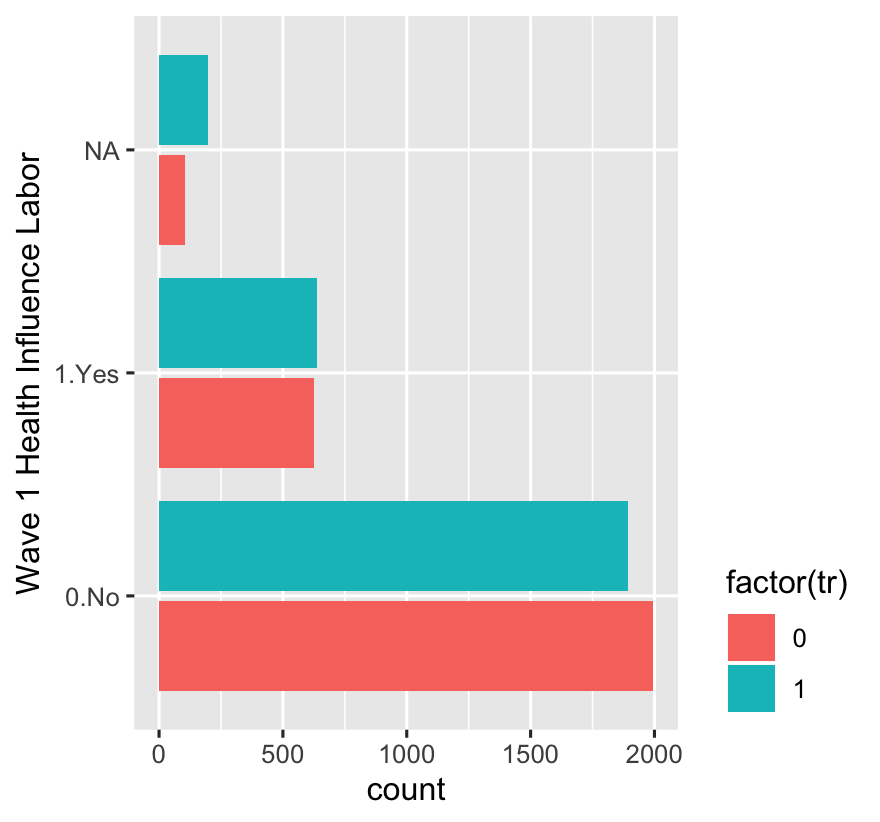
\includegraphics[width=6cm]{W1HealthLabor.png}
\end{minipage}
\begin{minipage}[t]{0.48\textwidth}
\centering
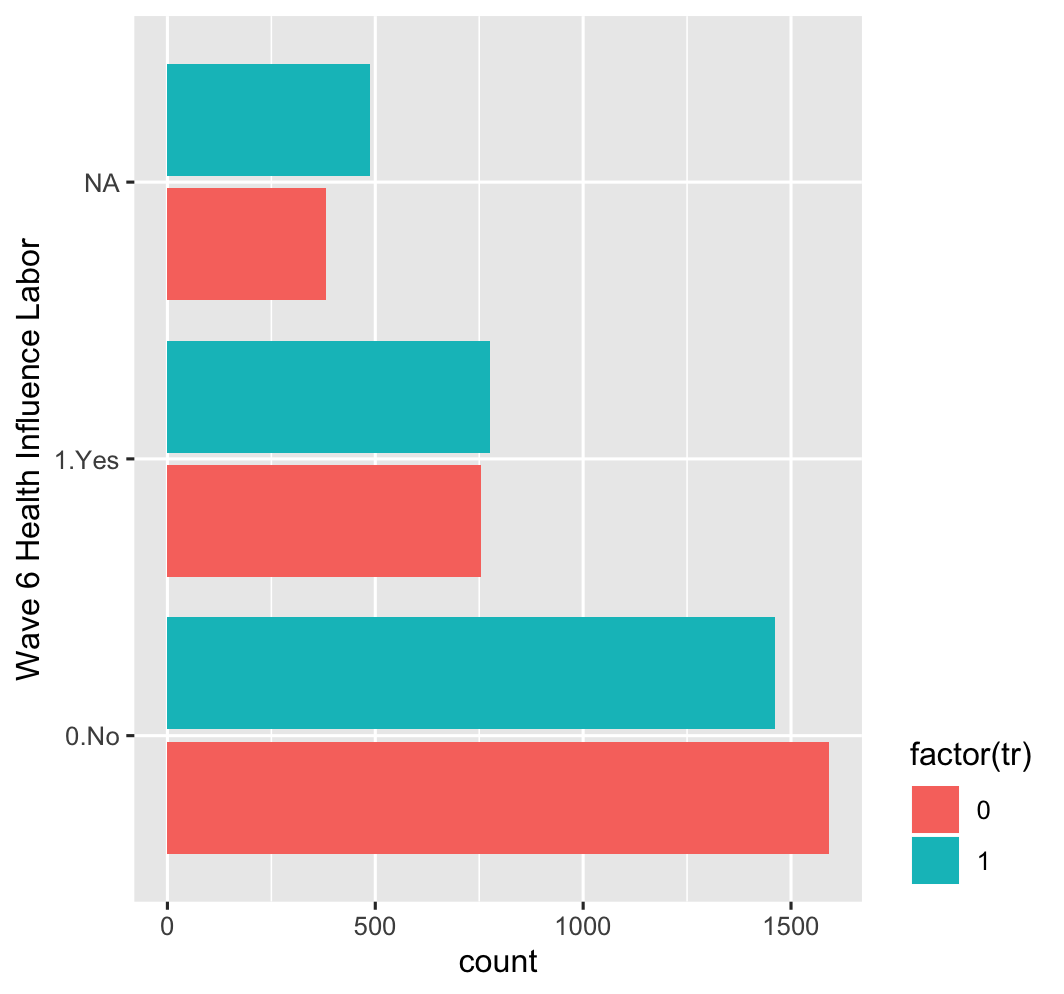
\includegraphics[width=6cm]{W6HealthLabor.png}
\end{minipage}
\caption{Health influence labor status for wave 1 and wave 6}
\end{figure}

\begin{figure}[htbp]
\centering
\begin{minipage}[t]{0.48\textwidth}
\centering
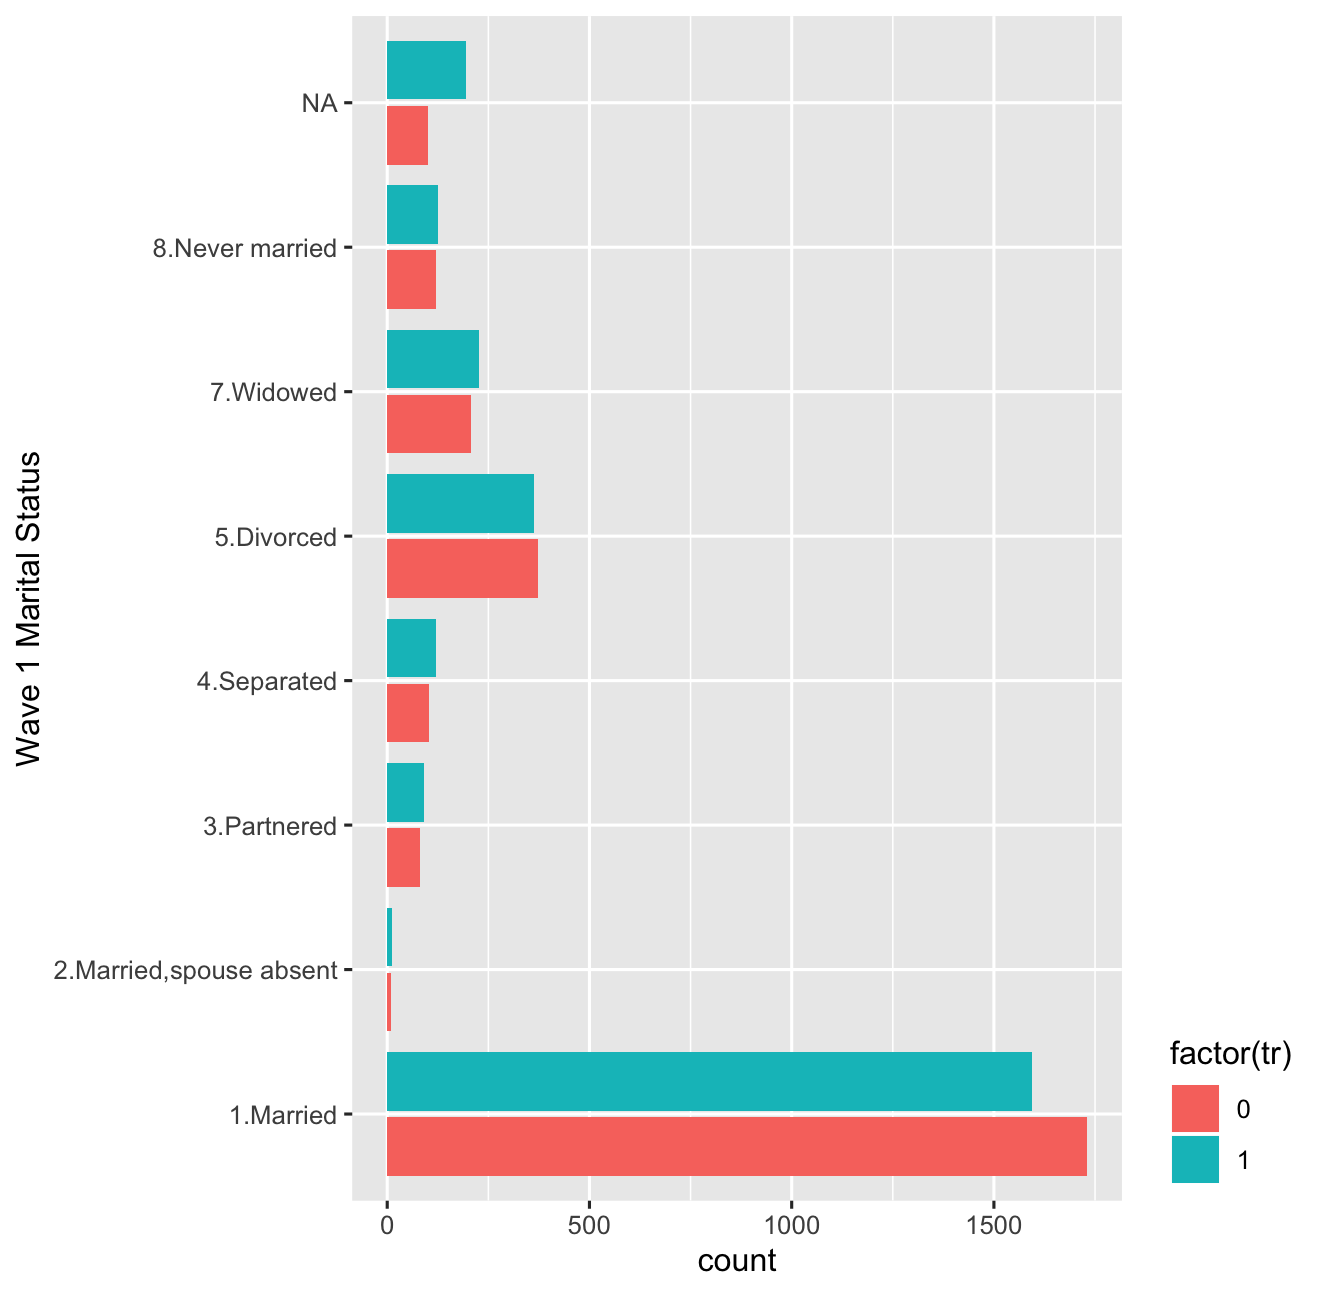
\includegraphics[width=6cm]{W1Marital.png}
\end{minipage}
\begin{minipage}[t]{0.48\textwidth}
\centering
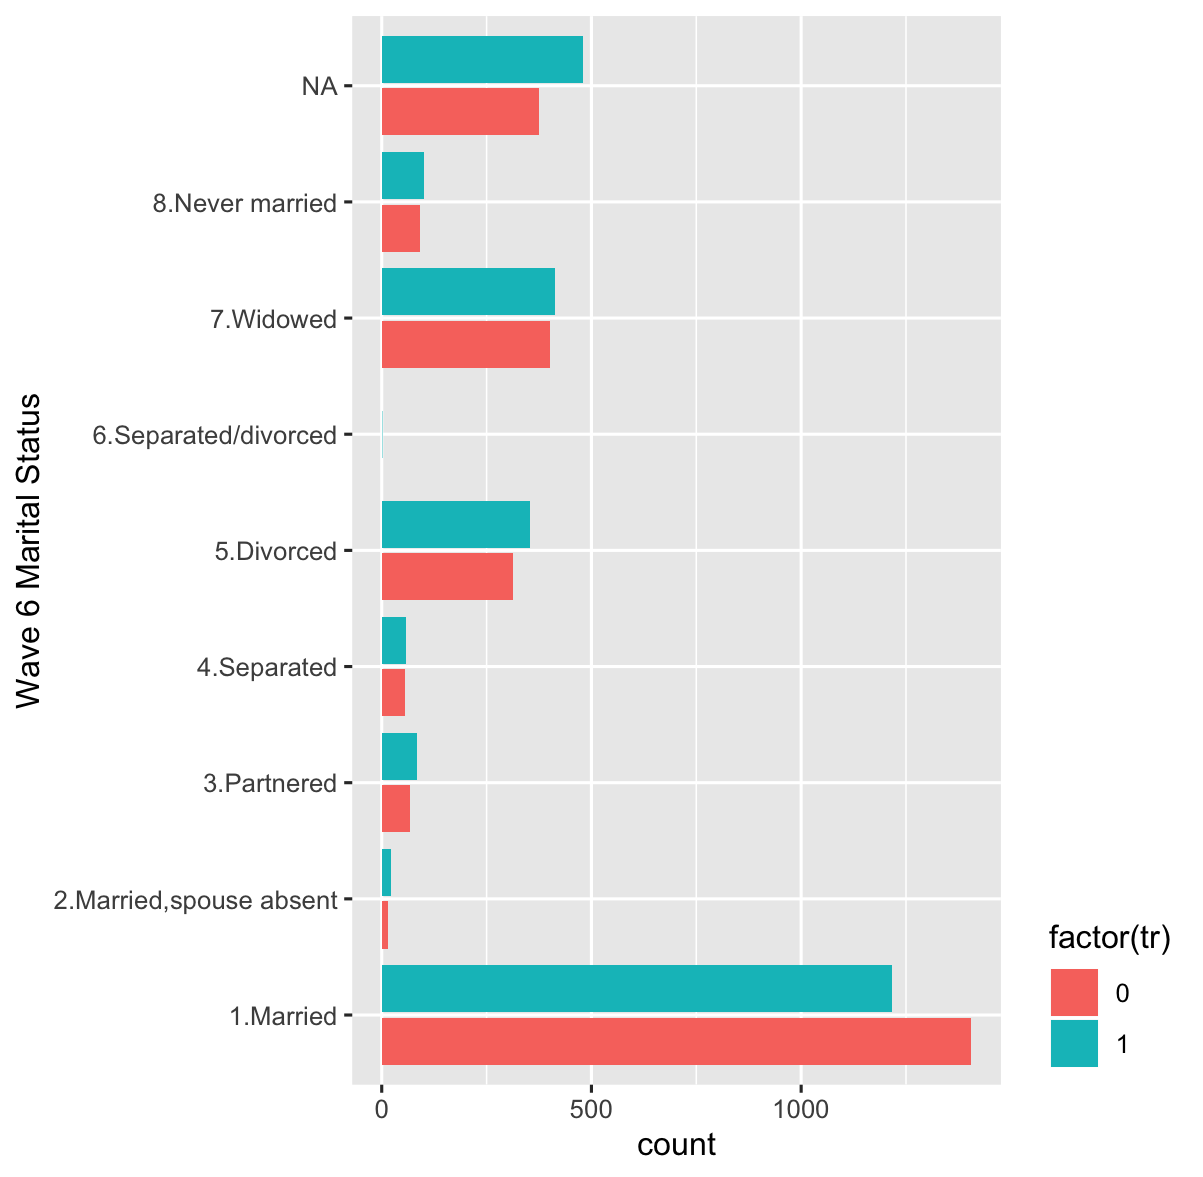
\includegraphics[width=6cm]{W6Marital.png}
\end{minipage}
\caption{Marital status for wave 1 and wave 6}
\end{figure}

These plots shows that the distribution of observed covariates are nearly identical between the treated and control groups. The matching algorithm works well.




\subsection{Statistical Analysis}
We perform a t test between the mortality rate among the treatment and control groups. The p-value of pairwise t-test is$ 1.07\times 10^{-7}$, with mean difference 0.031. So the treatment effect is significant.

\subsection{Sensitivity Analysis}
In the matching process, we paired two people with similar probability of being treated, which means $P_s$, which is the probability that the first subject of the sth pairs is the one who got treated, is nearly 0.5. The probability of experiencing negative wealth shock is unknown and can only be imputed by us. However, if there exists unobserved confounders, imputation could be inaccurate. So we perform the sensitivity analysis to test the robustness of our conclusion.

We got $\Gamma$ to be 1.59 and e-value is 2.83. So as long as $P_s$ is within $[0.39, \,0.61]$, the result still holds. So our conclusion is insensitive to unmeasured confounders.

\subsection{Heterogeneous Treatment effect}
There's one question remaining, is the treatment effect heterogeneous? We can compared the ATE among people with different characteristics.

\begin{table}[!ht] %[bhtp]
\centering
\caption{ATE among different gender}
\begin{tabular}{|c|c|}
\hline
Gender & ATE \\
\hline
All & 0.031 \\
\hline
Female & 0.031 \\
\hline
Male & 0.031 \\
\hline
\end{tabular}
\end{table}



\begin{table}[!ht] %[bhtp]
\centering
\caption{\textsl{ATE among people in different health condition}}
% \label{Table-3}
\begin{tabular}{|c|c|}
\hline
Health condition & ATE \\
\hline
All & 0.031 \\
\hline
Excellent & 0.018 \\
\hline
Very good & 0.011 \\
\hline
Good & 0.027 \\
\hline
Fair & 0.025 \\
\hline
Poor & 0.101 \\
\hline
\end{tabular}
\end{table}

\begin{figure}[!ht]
\centering
\includegraphics
[width=3in, height = 3in]
{ATE.png}
\caption{ATE among people in different ages}
\end{figure}

When we consider gender, ATE is homogeneous and is exactly the same among two genders. However, things is different about health condition. The effect of negative wealth shock is more significant among people in poorer health. This agrees with our common sense. Intuitively, people in bad health condition tend to be more fragile and vulnerable to large loss of money and sudden shock. The distribution of ATE among people in different ages is out of order and it's still heterogeneous. But this may be caused by limited sample size, so the conclusion is meaningless. 

In conclusion, the treatment effect is heterogeneous.



\section{Conclusion}
Considerable loss in income late in life cause an increase in all-cause mortality. Its effect varies among people in different health conditions, but is similar for females and males. Further research is needed to detect method to protecting old people through a serious personal economic crisis.












\begin{thebibliography}{9}


\bibitem{r8}
\textsc{Edin, K.} and \textsc{Reed, JM.} (2005).
\textit{Why don't they just get married? Barriers to marriage among the disadvantaged.}.
Future Child. 2005 Fall;15(2):117-37.

\bibitem{r5}
\textsc{Schneider, D.} (2011). 
\textit{Wealth and the Marital Divide}.
American Journal of Sociology, 117(2), 627–667.

\bibitem{r6}
\textsc{Haushofer, J.} (2011). 
\textit{On the psychology of poverty} and \textsc{Fehr, E.} (2014).
Science , 344 (2014), 862–867.

\bibitem{r7}
\textsc{Haushdofeasddadar, J.} (2011). 
\textit{On thwerre psycholoqwqweqeqewgy ogf poverty} and \textsc{Fehrsf, E.} (2014).
Sciencfwefe , 344 (2014), 8dfsfd62–867.

\bibitem{r3}
\textsc{Pool, L.} and \textsc{Burgard, S.} and \textsc{Needham, B.} and \textsc{Elliott, E.} and \textsc{Langa, K.} and \textsc{Leon, C.} (2018).
\textit{Association of a Negative Wealth Shock With All-Cause Mortality in Middle-aged and Older Adults in the United States.}.
AMA. 2018;319(13):1341-1350.

\bibitem{r1}
\textsc{Li, Y.} and \textsc{Propert, K.} and \textsc{Rosenbaum, P.} (2001).
\textit{Balanced Risk Set Matching.}.
Journal of the American Statistical Association 96, 870–882 

\bibitem{r2}
\textsc{Haviland, A.} and \textsc{Nagin, D.} and \textsc{Rosenbaum, P.} (2007).
\textit{Combining propensity score matching and group-based trajectory analysis in an observational study.}.
Psychological Methods, 12(3), 247–267.




\end{thebibliography}



% AOS,AOAS: If there are supplements please fill:
%\begin{supplement}[id=suppA]
%  \sname{Supplement A}
%  \stitle{Title}
%  \slink[doi]{10.1214/00-AOASXXXXSUPP}
%  \sdatatype{.pdf}" 
%  \sdescription{Some text}
%\end{supplement}


\end{document}
